\newpage
\subsection{Лабораторная работа №4. Транзакции}
Задачи к лабораторной работе №4:

На примере двух параллельных транзакций показать наличие или отсутствие одной из аномалий параллельного выполнения на выбранном уровне изоляции.

Для демонстрации выбраны уровень изоляции \texttt{READ COMMITTED} и аномалия <<неповторяющееся чтение>>. Требуется проверить, что произойдёт, если одна транзакция дважды читает одну и ту же строку таблицы \texttt{payment}, а между этими чтениями другая транзакция изменяет эту строку и фиксирует изменение. Если результаты двух одинаковых запросов различаются, аномалия присутствует на данном уровне изоляции.

Для проверки используется платёж с \texttt{payment\_id} = 125, исходная сумма которого равна 693.88. Изменение суммы не затрагивает значение \texttt{settlement\_id}, поэтому триггеры сводной таблицы значения счётчиков не меняют. Эксперимент выполнялся в двух сеансах \texttt{psql}: в первом выполнялась транзакция А, во втором --- транзакция Б.

\subsubsection{Сценарий}

Действия транзакции А представлены в листинге~\ref{lst:tx_a}, действия транзакции Б --- в листинге~\ref{lst:tx_b}.

\begin{lstlisting}[
    language=SQL,
    caption={Транзакция А},
    label={lst:tx_a}
]
BEGIN TRANSACTION ISOLATION LEVEL READ COMMITTED;

SELECT payment_id, payment_amount
FROM payment
WHERE payment_id = 125;

-- (транзакция Б изменяет и фиксирует данные)

SELECT payment_id, payment_amount
FROM payment
WHERE payment_id = 125;

COMMIT;
\end{lstlisting}

\begin{lstlisting}[
    language=SQL,
    caption={Транзакция Б},
    label={lst:tx_b}
]
BEGIN TRANSACTION ISOLATION LEVEL READ COMMITTED;

UPDATE payment
SET payment_amount = 1000.00
WHERE payment_id = 125;

COMMIT;
\end{lstlisting}

Порядок выполнения действий и их результаты представлены в таблице~\ref{tab:tx_scenario}.

\begin{table}[H]
\centering
\caption{Порядок выполнения сценария}
\label{tab:tx_scenario}
\small
\renewcommand{\arraystretch}{1.3} % Увеличивает вертикальные отступы в строках таблицы
\begin{tabularx}{\textwidth}{|c|X|X|}
\hline
\textbf{№} & \textbf{Действия транзакции А} & \textbf{Действия транзакции Б} \\ \hline
1 & \texttt{BEGIN TRANSACTION ISOLATION LEVEL READ COMMITTED;} & \\ \hline
2 & \texttt{SELECT payment\_id, payment\_amount FROM payment WHERE payment\_id = 125;} \par \textit{Результат:} \texttt{payment\_amount} = 693.88 & \\ \hline
3 & & \texttt{BEGIN TRANSACTION ISOLATION LEVEL READ COMMITTED;} \\ \hline
4 & & \texttt{UPDATE payment SET payment\_amount = 1000.00 WHERE payment\_id = 125;} \par \textit{Результат:} \texttt{UPDATE 1} \\ \hline
5 & & \texttt{COMMIT;} \\ \hline
6 & \texttt{SELECT payment\_id, payment\_amount FROM payment WHERE payment\_id = 125;} \par \textit{Результат:} \texttt{payment\_amount} = 1000.00 & \\ \hline
7 & \texttt{COMMIT;} & \\ \hline
\end{tabularx}
\end{table}

Скриншоты выполнения сценария представлены на рисунках~\ref{fig:lab4_tx_a} и~\ref{fig:lab4_tx_b}.

\begin{figure}[H]
    \centering
    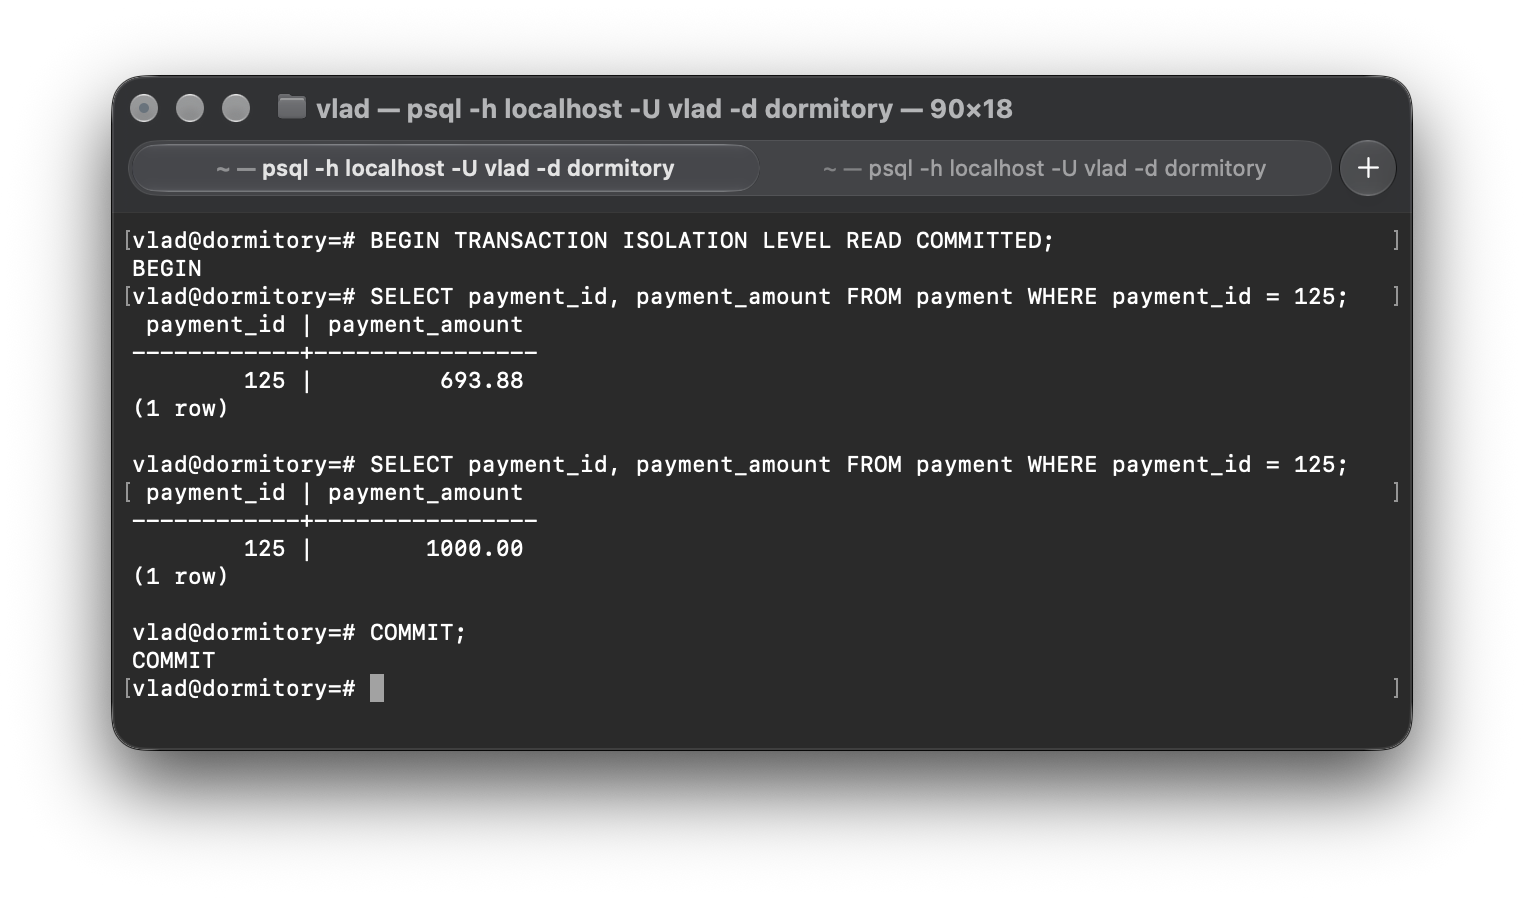
\includegraphics[width=1\textwidth]{figures/lab4_tx_a.png}
    \caption{Выполнение транзакции А}
    \label{fig:lab4_tx_a}
\end{figure}


\begin{figure}[H]
    \centering
    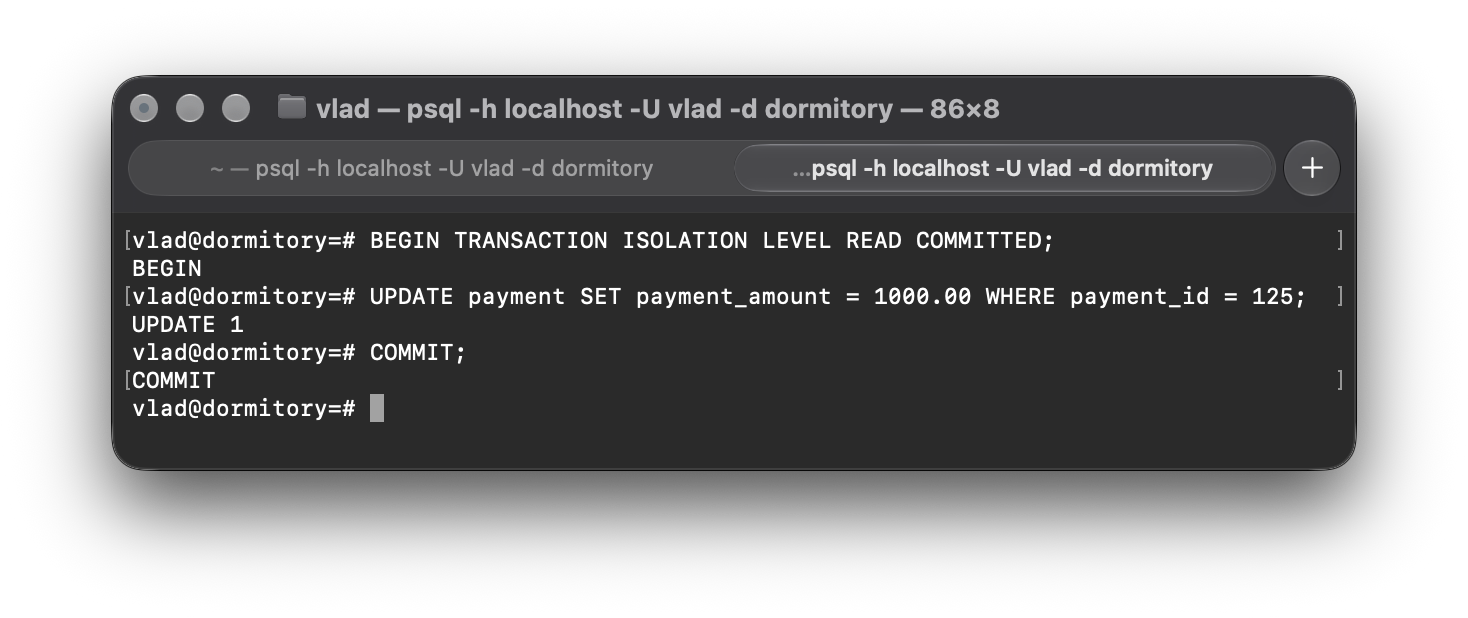
\includegraphics[width=1\textwidth]{figures/lab4_tx_b.png}
    \caption{Выполнение транзакции Б}
    \label{fig:lab4_tx_b}
\end{figure}

\subsubsection{Обоснование результата}

На уровне изоляции \texttt{READ COMMITTED} аномалия неповторяющегося чтения присутствует. Транзакция А дважды выполнила один и тот же запрос к строке с \texttt{payment\_id} = 125 и, не завершившись, получила разные значения: 693.88 при первом чтении и 1000.00 при втором. Это произошло потому, что между чтениями транзакция Б изменила сумму платежа и зафиксировала изменение командой \texttt{COMMIT}. На данном уровне каждый запрос видит все данные, зафиксированные к моменту его начала, а не к моменту начала транзакции, поэтому второй запрос транзакции А увидел результат работы транзакции Б. Для исключения такого поведения необходим уровень \texttt{REPEATABLE READ} или выше, при котором транзакция работает с единым снимком данных, зафиксированных к её началу.